\documentclass[12pt]{article}
\usepackage[utf8]{inputenc}

\usepackage{amsfonts}
\usepackage{amsmath}
\usepackage{bookmark}
\usepackage[a4paper, margin=3.5cm]{geometry}
\usepackage{graphicx} % For inserting images
\usepackage{hyperref} % For hyperlinks
\usepackage{indentfirst}
\usepackage{minted} % For code-highlighting
\usepackage{parskip}

\graphicspath{ {./images/} }
\setlength{\parindent}{15pt} % Set paragraph indentation
\setlength{\parskip}{1em} % Set paragraph space (one line)
\setminted{frame=single, breaklines} % Set codeblock style

\title{Programming Practicum Report:\\Meeting \#5}
\author{\href{https://github.com/avaxar}{R. Ethan Halim}}
\date{September 22nd, 2024}

\begin{document}

\maketitle

\section{Fizz Buzz}
The entire source file is hosted on a GitHub repository \href{https://github.com/avaxar/uni-practica-1/tree/main/week_5/01_fizz_buzz}{\textbf{here}}.

\subsection{Explanation}

As it is required to have the utilization of \texttt{std::vector} in the code, the vector used shall be to store the string of each value from 1 to 100 through the fizz-buzz algorithm. For performance, the \texttt{.reserve} method of \texttt{std::vector} is utilized, in order to avoid reallocations of the vector elements in the heap.

\begin{minted}{cpp}
int program(std::istream& cin, std::ostream& cout) {
    // Requirement: the use of std::vector
    std::vector<std::string> result;
    result.reserve(100); // So that the vector doesn't need to reallocate

    ...
}
\end{minted}

The for-loop below iterates from 1 to 100. In order to check whether the iterator \texttt{i} is a multiple of 3, 5, or both, the modulo operator \texttt{\%} is utilized to check the division remainder, whereby the result \texttt{0} signifies that the nominator is a multiple of the denominator. As the fizz-buzz algorithm needs to check the case where it is a multiple of both 3 and 5, the said condition shall precede the other two. \texttt{"FizzBuzz"}, \texttt{"Fizz"}, \texttt{"Buzz"}, or the decimal presentation of the number itself is then pushed into the \texttt{result} array.

\begin{minted}{cpp}
int program(std::istream& cin, std::ostream& cout) {
    ...

    for (int i = 1; i <= 100; i++) {
        // Both multiples of 3 and 5
        if (i % 3 == 0 && i % 5 == 0) {
            result.push_back("FizzBuzz");
        }
        // Only a multiple of 3
        else if (i % 3 == 0) {
            result.push_back("Fizz");
        }
        // Only a multiple of 5
        else if (i % 5 == 0) {
            result.push_back("Buzz");
        }
        // If neither
        else {
            result.push_back(std::to_string(i));
        }
    }

    ...
}
\end{minted}

Each element of the \texttt{result} array is then printed out one by one upon the conclusion of the algorithm.

\begin{minted}{cpp}
int program(std::istream& cin, std::ostream& cout) {
    ...

    // Prints each element in the final vector
    for (std::string& str : result) {
        cout << "- " << str << '\n';
    }

    return 0;
}
\end{minted}

\pagebreak
\subsection{Manual Testing}
Below is the compilation and the testing of the source code. The output is cut off to the 31st line, as the screenshot is unable to fit all 100 lines of the output.
\newline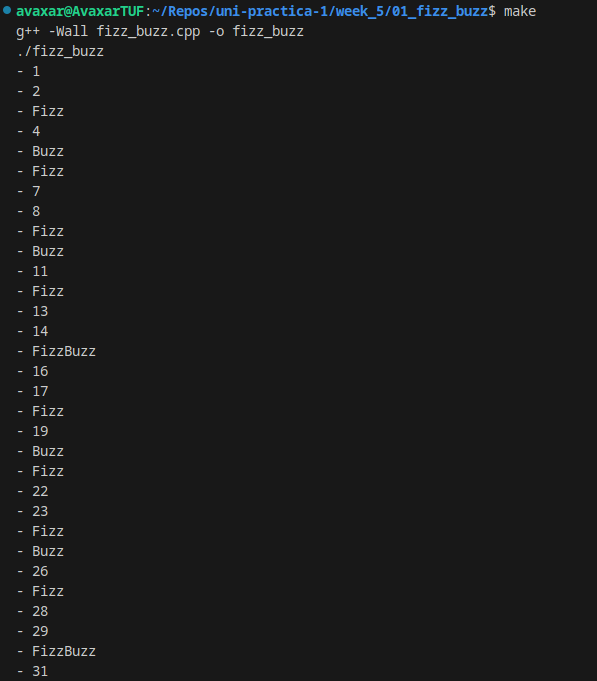
\includegraphics[width=\textwidth]{01_fizz_buzz}

\pagebreak
\subsection{Test Cases}

\subsubsection{Tests}
Below is copied directly from the \texttt{tests.txt} file.
\inputminted{text}{01_fizz_buzz/tests.txt}

\subsubsection{Execution}
Below are the results of the test cases. No test cases failed.
\newline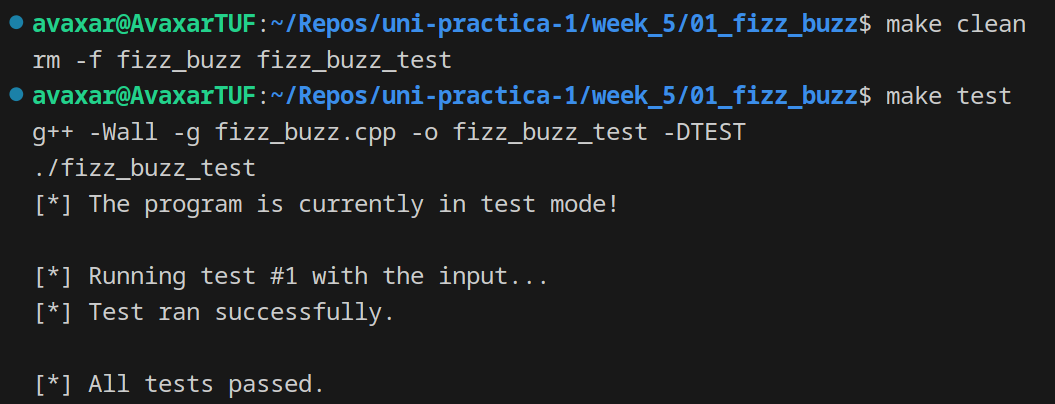
\includegraphics[width=\textwidth]{01_fizz_buzz_test}

\pagebreak
\section{Reversing a Vector}
The entire source file is hosted on a GitHub repository \href{https://github.com/avaxar/uni-practica-1/tree/main/week_5/02_reversal}{\textbf{here}}.

\subsection{Explanation}

First and foremost, the program has to accept a vector of integers as input from the user. This part of the code which comprises most of the source file handles the parsing of the vector input. As per what's desired, the vectors that are fed in are to be formatted as follows.
\begin{verbatim}
[1, 2, 3, 4, 5, ..., n]
\end{verbatim}
... where the vector begins with an opening square bracket and terminates with a closing square bracket, and the integer elements are comma-separated. Additionally, the algorithm to handle the parsing of such input string must take into factor extra whitespace. Therefore, it must also handle cases like as follows.
\begin{verbatim}
    [    1    ,    2    ,    3    ,    4    ,    5    ]
\end{verbatim}

I have provided brief explanations to each statement clause as comments in the code below. As an added auxiliary, the code checks for invalid syntax and informs the user thereof.

\begin{minted}{cpp}
int program(std::istream& cin, std::ostream& cout) {
    cout << "Input: ";
    std::vector<int64_t> vec;
    char inp;

    // Clears any whitespace
    do {
        cin >> inp;
    } while (std::isspace(inp));

    // Expects an opening square bracket for the vector
    if (inp != '[') {
        cout << "Expected an opening square bracket!\n";
        return 1;
    }

    // Clears any whitespace
    do {
        cin >> inp;
    } while (std::isspace(inp));

    // Loops until the array is closed
    while (inp != ']') {
        // The latter condition also handles negative numbers
        if (!('0' <= inp && inp <= '9') && inp != '-') {
            cout << "Expected a number, but instead saw '" << inp << "'!\n";
            return 1;
        }

        // Returns the checked character and reads for the integer
        cin.unget();
        vec.push_back(0);
        cin >> vec[vec.size() - 1];

        // Clears any whitespace
        do {
            cin >> inp;
        } while (std::isspace(inp));

        // Hints that the vector has ended
        if (inp == ']') {
            break;
        }

        if (inp != ',') {
            cout << "Expected a comma, but instead saw '" << inp << "'!\n";
            return 1;
        }

        // Clears any whitespace
        do {
            cin >> inp;
        } while (std::isspace(inp));
    }

    ...
}
\end{minted}
\pagebreak

Below is the actual part which deals with the reversal of the vector. The reversed content of the vector shall be stored in the variable \texttt{reversed}. The \texttt{.reserve} method of \texttt{std::vector} is utilized, in order to cull unnecessary reallocations of the elements in the heap upon appendage. The for-loop iterates backwards from \texttt{n - 1} (the index of the last element) to \texttt{0} (the index of the first element), in order to access the elements of \texttt{vec} in a similarly backwards manner, each of which is appended to the \texttt{reversed} vector.

\begin{minted}{cpp}
int program(std::istream& cin, std::ostream& cout) {
    ...

    // Reverses the vector
    std::vector<int64_t> reversed;
    reversed.reserve(vec.size()); // So that the vector doesn't need to reallocate
    for (size_t i = vec.size() - 1; i < vec.size(); i--) { // Iterates backwards
        reversed.push_back(vec[i]);
    }

    ...
}
\end{minted}

Finally, the program prints the resulted \texttt{reversed} vector and formats the vector properly, where the elements are enclosed in square brackets, and each element is separated in between each other with a comma.

\begin{minted}{cpp}
int program(std::istream& cin, std::ostream& cout) {
    ...

    // Prints the content of the reversed vector
    cout << "Output: [";
    for (size_t i = 0; i < reversed.size(); i++) {
        cout << reversed[i];
        if (i < reversed.size() - 1) {
            cout << ", ";
        }
    }
    cout << "]\n";

    return 0;
}
\end{minted}

\subsection{Manual Testing}
Below is the compilation and the testing of the source code.
\newline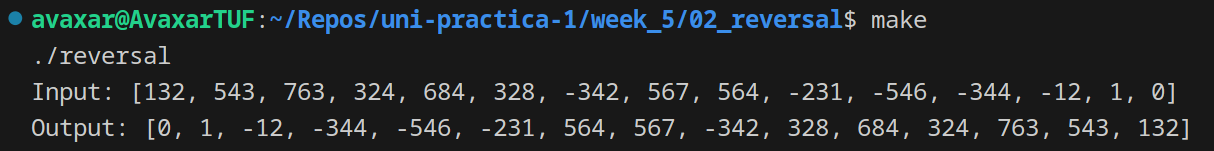
\includegraphics[width=\textwidth]{02_reversal}

\subsection{Test Cases}

\subsubsection{Tests}
Below is copied directly from the \texttt{tests.txt} file. The test cases test for scenarios, such as the lack of elements, a single element, multiple elements, multidigit elements, negative elements, and mixed blends of the said circumstances.
\inputminted{text}{02_reversal/tests.txt}

\subsubsection{Execution}
Below are the results of the test cases. No test cases failed.
\newline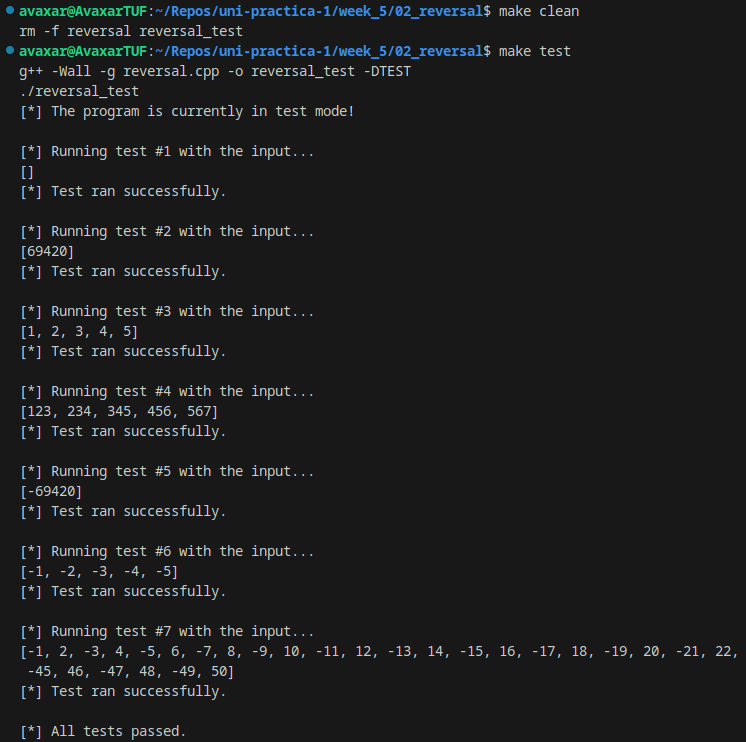
\includegraphics[width=\textwidth]{02_reversal_test}

\end{document}
